\documentclass[a4paper,11pt,twoside,openright]{book}
\usepackage[T1]{fontenc}
\usepackage[utf8]{inputenc}
\usepackage{lmodern}
\usepackage[spanish]{babel}
\usepackage{fancyhdr}
\usepackage{amsmath}
\usepackage{mathtools}
\usepackage{amssymb}
\usepackage{cite}
\usepackage{enumerate}
\usepackage{paralist}
\usepackage[linesnumbered,lined,boxruled,commentsnumbered,spanish]{algorithm2e}
\usepackage{graphicx}
\usepackage{float}
\usepackage[pdf]{graphviz}

\title{Título}
\author{Emiliano Roatta}

\begin{document}
\frontmatter

\maketitle

% begin "dedication"
\begin{flushright}
\null\vspace{\stretch{1}}
  Dedicatoria
\vspace{\stretch{3}}\null
\end{flushright}
% end "dedication"

\newenvironment{abstract}%
{\cleardoublepage\null\vfill\begin{center}%
\bfseries\abstractname\end{center}}%
{\vfill\null}

\begin{abstract}
  Lorem ipsum...
\end{abstract}


\tableofcontents
\listoffigures
\listoftables
\listofalgorithms

\mainmatter
\chapter{Introducción}
\section{Problema}

"Software ages as this social and organisational context evolves: teams change,
knowledge decays, documentation falls out of date, intentions and rationale are forgotten over time
(Ball and Eick, 1996)."

"Software development is a complex undertaking, involving a number of related tasks: specification,
design, implementation, testing, debugging, maintenance, modification, re-engineering. Each of those
tasks involves a number of cognitive demands, such as search, comprehension, analysis, problem
solving, representation. It’s no wonder that software development is so often described as complex.
The complexity derives from the nature of the problems addressed, the diversity of the tasks involved,
the nature of the artefacts produced, the changing social and organisational environment in which it is
conducted, and the impact of time on environment, needs, teams, and artefacts."\cite{PetreDeQuency06}

\section{Conceptos Preliminares}

\section{Solución}

\section{Contribución}
\subsection{Objetivos Generales}
\subsection{Objetivos Específicos}

\section{Organización del informe}
El presente informe se compone de una sucesión de 7 capítulos, organizados para introducir
el problema (Capítulo 1), establecer el marco teórico para darle soporte (Capítulos 2, 3 y 4),
presentar la herramienta que aporta una solución (Capítulo 5), comentar los experimentos y
las conclusiones obtenidas (Capítulos 6 y 7).

Dichos capítulos son descritos a continuación:

\paragraph[]{Capítulo 1: Introducción} Se determina el problema que da origen al informe,
junto con los conceptos premilinares y la solución propuesta.
Así mismo, se definen la contribución del presente trabajo junto con los objetivos generales
y específicos, y se presenta la organización correspondiente al informe.

\paragraph[]{Capítulo 2: Comprensión de Programas} \textit{TBD}

\paragraph[]{Capítulo 3: Métricas de Calidad en Software} Se revisa el estado del arte
en cuanto a las métricas de Calidad de Software, haciendo hincapié en las relacionadas al análisis
estático de código.

\paragraph[]{Capítulo 4: Análisis de Identificadores} Se ahonda sobre los conceptos relacionados
a los indicadores y sus propiedades; y se recorren con detalle los algoritmos para el procesamiento
de los mismos, tanto para división como expansión.
Se explica cada uno de los algoritmos, haciendo énfasis en los implementados en el presente trabajo.

\paragraph[]{Capítulo 5: Herramienta} Se presenta la herramienta, describiendo su estructura y
el proceso completo desde el análisis de código hasta la obtención de las métricas de interés.
También se explican las particularidades del lenguaje soportado por la herramienta.

\paragraph[]{Capítulo 6: Experimentos y Resultados} Se determinan cuáles fueron los experimentos
realizados, así como también los resultados de los análisis de los mismos.

\paragraph[]{Capítulo 7: Conclusiones} Se presentan las conclusiones extraídas 
después de la ejecución de los experimentos y el análisis de los resultados.
Además, se plantean trabajos futuros a partir del actual.


\chapter{Calidad de Software}
\section{Introducción}

Un aspecto muy importante dentro de la disciplina de desarrollo de software, tanto
a nivel de \textit{producto} como de \textit{proceso}, es la \textbf{calidad del
software}.
Ésta determina el grado en el que un producto satisface los requerimientos de sus usuarios
tanto internos como externos, y cómo les aporta valor a los mismos.

Se considera que un \textit{modelo de calidad} tiene el objetivo de describir, evaluar y/o
predecir la calidad de un componente \cite{Wagner2013}; y a lo largo de las últimas cuatro
décadas se han propuesto diferentes y diversos modelos \cite{Deissenboeck2009}.
Dentro de este conjunto de diversas propuestas podemos encontrar: modelos taxonómicos, como
lo es la familia de normas ISO/IEC 25000 \cite{ref}; modelos basados en métricas como el
índice de mantenibilidad (MI) \cite{ref}; modelos estocásticos, como los modelos de crecimiento
de confiabilidad (RGMs) \cite{ref}.

El problema existente con los tipos de modelos nombrados anteriormente viene dado por sus
diferentes propósitos.
La familia de normas ISO/IEC 25000 tiene como objetivo principal \textit{definir} lo que
corresponde a calidad en un sistema; mientras que un esquema orientado a métricas como MI
pretende \textit{evaluar} el nivel de calidad; mientras que los modelos de crecimiento de
confiabilidad se utilizan para \textit{predecir} la calidad.

Si bien los diferentes modelos se caracterizan por un objetivo particular, ya sea de
\textit{definición}, \textit{evaluación} o \textit{predicción}, éstos no son independientes,
debido a que es muy difícil evaluar calidad sin una propia definición de la misma, como también
es muy difícil predecir un determinado nivel de calidad sin saber cómo evaluarlo.

AGREGAR ENGANCHE CON MANTENIBILIDAD.
Cuál sería?

\section{Mantenibilidad}

\subsection{Definición}

Uno de de los modelos enfocados en la definición de calidad y sus diferentes aspectos
viene establecido por la familia de normas ISO/IEC 25000 \cite{ref}, 
la cual provee guías para obtener un producto de calidad, mediante la especificación 
de requisitos y características de calidad, así como la evaluación de las mismas.
Esta familia de normas está basada en dos normas anteriores (ISO/IEC 9126 \cite{ref}
e ISO/IEC 14598 \cite{ref}), y presenta cinco divisiones, las cuales se enfocan en diferentes
elementos y su proceso.

Particularmente, la norma ISO/IEC 25010, describe el modelo de calidad tanto para el producto
final como para el uso del mismo; definiendo así las características y subcaracterísticas
utilizadas en la evaluación de un elemento, siendo éstas:
\begin{inparaenum}[(1)]
    \item Adecuación funcional,
    \item Eficiencia de desempeño,
    \item Compatibilidad,
    \item Usabilidad,
    \item Fiabilidad,
    \item Seguridad,
    \item Mantenibilidad y
    \item Portabilidad.
\end{inparaenum}
Particularmente, la característica de \textbf{Mantenibilidad} representa la \textit{capacidad del
software para ser modificado de forma eficiente y efectiva, ya sea por motivos correctivos,
evolutivos o perfectivos}.

Así mismo, Mantenibilidad está compuesta por cinco subcaracterísticas:
\begin{inparaenum}[(a)]
    \item Modularidad,
    \item Reusabilidad,
    \item Analizabilidad,
    \item Capacidad para ser modificado \textit{(Modificabilidad)} y
    \item Capacidad para ser probado.
\end{inparaenum}
En el contexto de este trabajo, las subcaracterísticas de mayor interés corresponden
a la \textit{Analizabilidad} y la \textit{Modificabilidad}.
La \textbf{Analizabilidad} está asociada a la facilidad con la que se pueden diagnosticar problemas
o fallas en el software, identificar las partes/componentes de un sistema a modificar, y la
evaluación del impacto generado por los cambios.
Por otro lado, la \textbf{Modificabilidad} viene dada por la capacidad del producto para ser
modificado de forma efectiva y eficiente, sin introducir defectos o afectar la performance.

\subsection{Evaluación}

Así como la familia de normas ISO/IEC 25000 define un conjunto de características y
subcaracterísticas, también provee un listado básico de métricas para su medición.
Este listado no es exhaustivo, ya que se pueden emplear métricas no definidas por el
estándar, siempre y cuando se determine su correlación con alguna de las características
establecidas.
En la tabla \ref{Metrics} se listan las métricas definidas por el estándar, para la \textit{Mantenibilidad}
y sus subcaracterísticas.

\begin{figure}
    \label{Metrics}
    \includegraphics[width=12cm]{quality_metrics/quality_metrics.png}
    \centering
    \caption{Métricas para Mantenibilidad y su subcaracterísticas}
\end{figure}

Sin embargo, este conjunto de normas como otras existentes o anteriores sólo ofrecen una
guía muy abstracta sobre la definición de calidad de software, y no indican cómo lograr
que el software sea de calidad, ni cómo hacer una correcta medición \cite{Relf04}.
Al igual que los primeros modelos escritos a finales de la década de 1970, como los
propuestos por Boehm et al. \cite{Boehm1978} y McCall et al. \cite{McCall1977}, los cuales trataban
de definir la calidad de software como una descomposición jerárquica de características y
subcaracterísticas.

Por lo tanto, la investigación subsiguiente se enfocó principalmente en encontrar maneras de
cuantificar las propiedas definidas por los estudios anteriores.
Los trabajos de Dromey \cite{Dromey1995} y de Bansiya y Davis \cite{Bansiya2002}, son los más 
importantes ya que forman la base sobre la cual se construyeron los modelos más recientes, al 
describir cómo los atributos de alto nivel de calidad pueden medirse a partir de \textit{propiedades
de bajo nivel}, cuantificadas desde \textbf{métricas de software y análisis estático}.

Las contribuciones más significativas en el campo de la \textit{evaluación cuantitativa de la calidad},
basadas en el \textbf{análisis estático de código fuente} vienen dadas por el Modelo de Mantenibilidad 
SIG \cite{Heitlager2007}, junto con Quamoco tool chain \cite{Wagner2012}.

\subsubsection{Modelo de Mantenibilidad SIG}

Este modelo de evaluación de calidad \cite{Heitlager2007} permite determinar la mantenibilidad
de un proyecto de software, donde las características son descompuestas en un
conjunto de subcaracterísticas, y estas últimas en \textit{propiedades}.
Estas propiedades son cuantificables directamente desde el código fuente del producto, utilizando
análisis estático, permitiendo que a partir de estos valores junto con unos determinados umbrales,
cada propiedad reciba un \textit{perfil de calidad}.

Al poder cuantificar estas propiedades y obtener los perfiles, también se pueden agregar,
y de esta manera establecer un puntaje global de calidad del sistema.
Con el fin de mantener la objetividad en los umbrales para la evaluación de propiedades,
estos son obtenidos a través de benchmarking \cite{Alves2010}.

\subsubsection{Quamoco Tool Chain}

Similar al Modelo de Mantenibilidad SIG \cite{Heitlager2007}, Quamoco Tool Chain \cite{Wagner2012}
se basa en propiedades extraídas desde el código fuente a través de análisis estático del mismo,
con la diferencia de que permite a los interesados definir sus propios modelos jerárquicos
de calidad.

Quamoco define un meta-modelo, facilitando la creación de modelos más genéricos, en lugar de
estar restringidos a ciertos atributos de calidad como lo es la mantenibilidad, al introducir
el elementos que permiten cerrar la brecha entre medidas concretas y aspectos abstractos de
calidad.
Toma como base los atributos de calidad definidos en la norma ISO 25010, pero los refina
aplicando 200 factores y 600 mediciones para sistema Java y C Sharp.

\subsection{Predicción}

\textit{TBD}

\section{Impacto de los identificadores en Calidad de Software}

"The impact of low quality identifier names on program comprehension is reasonably
well understood \cite{DeiBenbockPizka05,Lawrie2007,Lawrie2006}, but little is known
about the extent to which the quality of identifier names might influence the quality
of source code" \cite{ButlerWemelingerYu10}.

"Buse and Weimer \cite{Buse2008} developed a readability metric for Java derived from measurements 
of, among others, the number of parentheses and braces, line length, the number
of blank lines, and the number, frequency and length of identifiers.
Using machine learning, the readability metric was trained to agree with the judgement 
of human source code readers.
Buse and Weimer found a significant statistical relationship between the readability of 
methods and the presence of defects found by FindBugs in open source code bases. 
Although their work makes a link between readability and software quality, their notion
of readability ignores the quality of identifier names".

Se ignora el contenido semántico.

"The predictive probability associated with each relationship illustrates the utility
of the identifier flaws as light-weight classifiers for source code quality"
\cite{ButlerWemelingerYu10}.

\textbf{"a low-cost heuristic to identify potentially problematic regions of source code"}

"Software quality is not defined in terms of quality attributes but instead must be
inferred from characteristics that correlate to quality attributes and defect attributes.
One of these quality attributes is the readability of the software.
However, the software engineer, who is ultimately responsible for software quality,
is not supported well by their formal education, the software engineering culture, the
existence of useful tools and where these tools do exist by their limited up-take by industry.
Human cognitive limitations similarly frustrate the development of readable source code.
Software characteristics have been identified, which correlate well to source code readability.
One of these software characteristics, which have been supported by empirical research,
is the choice of identifier name".\cite{Relf04}

"A software characteristic that has the potential to improve software quality is the choice of
identifier name, and this is particularly so in large software systems.
identifier-naming sytle guidelines, supported by empirical evidence and generally accepted by
software professionals to direct towards improved source code readabiity are candidates for
automation by a tool.
Such an automated tool could make visibile aspects of software quality that are less keenly
perceived by the novice programmer and could assist in ther education along the path to
expert status"\cite{Relf04}.

"Existing research on source code readability focuses on the contribution the
components of source code make to readability" \cite{Buse2008}.


\chapter{Comprensión de Programas}
\section{Introducción}

La \textit{Comprensión de Programas} es una disciplina de la Ingeniería de Software
cuyo objetivo es proveer \textit{Modelos, Métodos, Técnicas} y \textit{Herramientas}
para facilitar el estudio y entendimiento de los sistemas de software \cite{BeronHenriquesPereira10}.

La importancia de la Comprensión de Programas radica en que es una de las demandas cognitivas
más importantes, dentro del conjunto necesario para llevar adelante las tareas implicadas
en el proceso de desarrollo y sus distintas fases \cite{PetreDeQuincey06}.
La correcta aplicación de los modelos, métodos, técnicas y herramientas propuestas por
la Comprensión de Programas, hacen que el desarrollador pueda localizar y entender rápidamente
los elementos empleados para soportar una funcionalidad específica, disminuyendo el tiempo requerido
para la realización de una tarea, impactando positivamente en los costos asociados a la
modificación, mantenimiento y evolución de un sistema \cite{BeronHenriquesPereira10}.

La forma que tienen los programadores de entender un sistema, componente o pieza de código fuente
puede ser descrita a través de diferentes modelos, los cuales componen la base para las herramientas
de comprensión de programas \cite{BeronHenriquesPereiraUzal07}.
Éstos son denominados \textit{modelos cognitivos}.
La información necesaria para aplicar los modelos cognitivos, se obtiene a través de
\textit{métodos de extracción de la información}.
Para facilitar la compresión y el proceso establecido en el modelo cognitivo, se utilizan
diferentes técnicas de \textit{visualización de software}, y así procesar mejor la
información extradía por distintos métodos.
Por último, diferentes \textit{estrategias para la inter-conexión de dominios} pueden ser
aplicadas para que el programador asocie el dominio del problema, con el dominio
del programa bajo estudio.

Las siguientes secciones, desarrollan sobre los conceptos nombrados previamente.

\section{Modelos de Comprensión de Programas}

Generalmente se establece que la \textit{comprensión}, dentro de este ámbito de estudio, es un
proceso en el que el individuo construye su propia representación mental de un programa.
Si bien existen varias escuelas de pensamiento, independientemente de las diferencias, la
mayoría de los modelos de comprensión de programas contiene un conjunto común de elementos,
tal como se puede ver en la Figura X \cite{SchulteClear10}.

\begin{figure}[H]
    \includegraphics[width=10cm]{program_comprehension/elements.png}
    \centering
    \caption{Elementos principales de los modelos de comprensión de programas}
\end{figure}

\subsection{Representación Externa}
Se considera que la representación externa son todos aquellos materiales asociados al programa
en estudio que el programador puede utilizar para su proceso de comprensión, pero que no son 
parte del conocimiento interno del individuo.
Estos elementos pueden ser presentados de diversa forma, incluyendo directamente el código fuente,
hasta manuales, documentación, diagramas UML, entre otros.

\subsection{Estructura Cognitiva}
El conocimiento interno de un programador, el cual puede dividirse entre base de conocimiento
y representación mental, es lo que se define como estructura cognitiva.

La base de conocimiento viene dada por el conocimiento general que el programador posee,
independiente de la aplicación específica que se está tratando de comprender.
Esto incluye conocimiento general de lenguajes y principios de programación, algoritmos, 
aplicaciones similares y demás.

El modelo mental es una representación interna al programador del software bajo consideración.
Determina el nivel de conocimiento del individuo sobre el sistema en cuestión, y es construido
a medida que se comprende, utilizando la base de conocimiento mencionada anteriormente.
Diferentes elementos, tanto estáticos como dinámicos, forman parte del modelo y permiten
su evolución.\cite{MayrhauserVans95}

\subsection{Proceso de Asimilación}
La estrategia implementada por los desarrolladores para extraer información de un programa, 
construir una representación mental del mismo, y así lograr su comprensión, es lo que se
conoce como proceso de asimilación.

\begin{description}
    \item[Top-down] Los modelos de comprensión top-down son aquellos que implican la
    aplicación de conocimiento sobre el dominio del programa y la correlación de este
    conocimiento con el código fuente del mismo.
    En el modelo de Brooks, una sucesión de hipótesis forma el proceso de asimilación.
    En el esquema de Soloway y Erlich, los programadores utilizan planes y reglas de programación
    para descomponer objetivos y planes en otros planes de menor abstracción.
     
    \item[Bottom-up] Caen dentro de esta clasificación aquellos modelos en
    los que su proceso de asimilación comienza con las sentencias de código fuente, y
    las mismas se van agrupando y así obteniendo mayores niveles de abstracción.
    El proceso se repite una y otra vez, hasta lograr una representación mental completa
    del programa en cuestión.
    En el proceso de asimilación propuesto por Pennington, se presentan dos modelos diferentes.
    El modelo del programa, que se obtiene de agrupar microestructuras en macroestructuras, y
    se corresponde con una abstracción del flujo de control del programa.
    El modelo de situación, incluye el flujo de datos dentro del programa, y representa la
    función y objetivos del mismo.
    En el modelo de Shneiderman y Mayer, la base de conocimiento se compone tanto de
    conocimiento sintáctico como semántico.
    A mayor experiencia del desarrollar, mayor será este último.

    \item[Oportunista] Algunos autores consideran que, dependiendo
    de la necesidad de comprensión para la tarea en cuestión, no existe un enfoque
    sistemático de resolución.
    Algunos autores consideran que no existe un enfoque sistemático de asimilación,
    y que dependiendo de la necesidad de comprensión, un programador puede aprovechar
    las estrategias tanto bottom-up como top-down.
    Letovsky plantea que un programador puede procesar la información de forma bottom-up
    o top-down a medida que van apareciendo pistas que ayuden a su comprensión.
    
    \item[Modelos Integrados] Los modelos integrados suponen una combinación de los
    anteriores, en donde el proceso de asimilación implica ir cambiando de
    modelos a medida que se requiera, para poder construirlos simultáneamente.
    Se plantean tres representaciones mentales: el modelo del dominio, el modelo del
    programa y el modelo de situación.
    Es muy importante la base de conocimiento del programador, ya que le va a permitir
    la construcción de las representaciones.

\end{description}

\section{Métodos de Extracción de la Información}

Para poder lograr comprender una pieza de código fuente o programa bajo estudio, un
programador debe ser capaz de poder obtener información del mismo.
El tipo de información que el usuario necesita, depende de la tarea que tenga que llevar
adelante respecto al software.
Dentro la disciplina de Comprensión de Programas, para extraer la información requerida 
por los diferentes procesos cognitivos, se utilizan dos tipos de análisis:
\textit{Análisis Estático} y \textit{Análisis Dinámico}.

El \textbf{análisis estático} del software consiste en obtener información sobre el 
sistema de interés, pero sin ejecutarlo \cite{Binkley07}.
Los \textit{analizadores sintácticos} operan a nivel de código fuente, empleando
técnicas tanto de \textit{pattern matching} como de construcción de árboles de sintáxis
abstracta (\textit{Abstract-Syntax Tree}).
Los \textit{analizadores semánticos} trajaban de una manera diferente, ya que consideran
la secuencia en la que pueden darse los estados de un programa, en una ejecución.
La premisa principal consiste en que analizar los posibles estados de un programa en un
punto determinado, son suficientes para probar propiedades estáticas del mismo.
\cite{Cousot77}

El \textbf{análisis dinámico} corresponde a la extracción de propiedades de un sistema
en ejecución, empleando diferentes técnicas.
La \textit{instrumentación de código} es una de éstas, y permite obtener información sobre
las llamadas realizadas a una función dentro de una traza, junto con su contexto.
Es importante destacar que hay que identificar los aspectos de interés para el análisis,
y así reducir el overhead que trae aparejado esta técnica.
Los resultados tienen una gran precisión, pero sólo se garantizan para un conjunto particular
de datos de entrada, ya que es muy dependiente del input \cite{Ball99}.

La tabla \refeq{tab:dinamyc_static_analysis} muestra una comparativa \cite{GosainSharma15} 
entre los dos tipos de análisis, los cuales extraen información que luego debe ser
accedida e interpretada a través de distintas herramientas de visualización.

\begin{table}[]
    \caption{Comparación entre análisis estático y dinámico}
    \label{tab:dinamyc_static_analysis}
    \begin{tabular}{ll}
        \hline
        \textbf{Análisis Dinámico}             & \textbf{Análisis Estático}        \\ \hline
        Requiere que el programa sea ejecutado & No requiere ejecuciones           \\
        Mayor precisión                        & Menor precisión                   \\
        Válido para una ejecución particular   & Válido para todas las ejecuciones \\
        \begin{tabular}[c]{@{}l@{}}Adecuado para manejar características \\ de los lenguajes en tiempo de ejecución \\ (polimorfismo, hilos, enlaces dinámicos)\end{tabular}              & \begin{tabular}[c]{@{}l@{}}Carece de manejo de características \\ de los lenguajes en tiempo de \\ ejecución\end{tabular}         \\
        \begin{tabular}[c]{@{}l@{}}Implica mayor overhead en tiempo \\ de ejecución\end{tabular}              & No implica overhead               \\ \hline
    \end{tabular}
\end{table}

\section{Visualización de Software}

La visualización de software refiere al uso de diversos elementos (texto, 
gráficos 2D y 3D, diagramas, imágenes, vídeos, entre otros) para representar algún
aspecto de un programa y facilitar su comprensión \cite{PetreDeQuincey06,Chen06,GomezHenriquez01}.
Estos aspectos u objetos de interés pueden ser abstracciones de componentes, de
un sistema completo e incluso del comportamiento en tiempo en ejecución de los
mismos \cite{TeysereCampo09}.

Las visualizaciones pueden ayudan al programador durante tres procesos cognitivos
\cite{ButlerAlmond93}:
\begin{enumerate}[a)]
    \item \textit{proceso de descubrimiento o exploratorio}, en donde el usuario no
    sabe específicamente qué está buscando;
    \item \textit{proceso de toma de decisión o analítico}, en el cuál el usuario sabe lo que
    está buscando y sólo necesita encontrarlo;
    \item \textit{proceso descriptivo}, en el cuál es conocido el patrón que aparece en los
    datos pero necesita una visualización acorde para expresarlo.
\end{enumerate}

Los procesos cognitivos enumerados anteriormente suelen emplearse en diferentes tareas 
que puede llevar a cabo un programador.
Dentro de esta lista de tareas \cite{MalleticMarcusCollard02} encontramos: desarollo,
debugging, pruebas, mantenimiento y detección de errores, re-ingeniería, ingeniería reversa,
administración del proceso de software, y marketing.
En las primeras etapas del desarrollo de un nuevo sistema o aplicación, las visualizaciones
permiten la colaboración entre desarrolladores, y de esta manera ayudar en la definición y 
validación de los requerimientos.
A medida que se avanza en la construcción del software, las herramientas permiten validar
los avances y encontrar defectos.
En el caso de mantenimiento, ayudan en la comprensión del programa, en el entendimiento 
de su diseño y el planteo de su evolución \cite{PetreDeQuincey06}.

Algoritmos, programas y sistemas son los diferentes alcances que se consideran
dento de la disciplina de Visualización de Software \cite{PriceBaeckerSmall93,Myers90}.
La \textit{visualización de sistemas} se emplea para representar el sistema en su conjunto,
a través de los diferentes módulos que lo componen.
En la \textit{visualización de programas}, se busca mostrar el comportamiento de los mismos
y la relación entre sus componentes \cite{BenAri01}.
Por último, la \textit{visualización de algoritmos} se utiliza principalmente en el campo 
de la enseñanza, para demostrar el funcionamiento de algoritmos y estructuras de datos.
Así mismo, tal como denota la expresión 
\begin{center}
    $Alg. Visualization \subseteq Prog. Visualization \subseteq System Visualization$
\end{center}
las técnicas implementadas en un determinado alcance, pueden ser implementadas
también en un conjunto de mayor nivel de abstracción \cite{BeronHenriquesPereiraUzal07}.

La taxonomía de Price, Baecker y Small \cite{PriceBaeckerSmall93}, establece que
existen seis categorías de atributos para los sistemas de visualización.
Dentro de las mismas podemos encontrar:
\begin{enumerate}
    \item \textbf{Alcance:} dado por el espectro de programas que pueden ser analizados.
    \item \textbf{Contenido:} correspondiente al conjunto de propiedades del sistema que se 
    pueden extraer y visualizar.
    \item \textbf{Forma:} relacionado a la salida de los resultados de la visualización.
    \item \textbf{Método:} determinado por cómo está especificada la visualización.
    \item \textbf{Interacción:} referida la manera en la que el usuario pueda controlar e
    interactuar con la visualización.
    \item \textbf{Efectividad:} grado de adecuación con el cual se comunica la información
    al usuario.
\end{enumerate}
Del listado anterior, la categoría y por lo tanto la característica más importante corresponde
a la \textit{efectividad}.

La visualización de la información, extraída tanto de forma estática como dinámica,
es necesaria para ayudar al modelo de comprensión de programas en el procesamiento de
de la misma.
De esta manera, los distintos componentes facilitan la difícil tarea de
interconectar los dominios del problema y el programa.

\section{Estrategias de Interrelación de Dominios}

En las secciones anteriores se describen modelos cognitivos, características de
visualizaciones e incluso formas de extraer información para soportar estos 
procesos y/o elementos.
Si bien todos estos forman parte de la disciplina de Comprensión de Programas, hacen
hincapié principalmente en la comprensión del Dominio del Programa.
Al considerarse que un programador comprende completamente un sistema cuando puede
relacionar la funcionalidad que provee con los componentes del sistema y el código
fuente que lo ejecuta, es necesario tender los puentes entre el \textit{Dominio del Problema}
y el \textit{Dominio del Programa}.

\begin{figure}[H]
    \includegraphics[width=6cm]{program_comprehension/domains.png}
    \centering
    \caption{Interrelación de Dominios}
\end{figure}

Existen diferentes estrategias\cite{BeronOliveiraCruz10} para este proceso de 
\textit{inter-relación de dominios}.
Los mismos son explicados brevemente a continuación:

\paragraph{SVS (Simultaneous Visualization Strategy)}
En esta estrategia, se utiliza información extraída dinámicamente, a través de
la instrumentación del código fuente.
Un inspector, insertado durante la instrumentación, extrae información de las funciones 
que son ejecutadas; mientras que el monitor se encarga de mostrar esta información.
De esta manera, mediante la ejecución y observación, el programador puede relacionar
el Dominio del Problema con el Dominio del Programa. 

\paragraph{BORS (Behavioral-Operational Relation Strategy)}
Al igual que la SVS, en esta estrategia también se utiliza instrumentación del código,
para extraer información del árbol de llamada de funciones.
Esta estrategia se plantea en tres pasos.
En el primero, de índole observacional, se identifican los objetos del dominio y sus interfaces,
los cuales a través de algunas técnicas son extraídos y puestos en una lista.
El segundo paso, a través de la ejecución del código ya instrumentado, construye el árbol de
llamadas.
El tercer y último paso, consiste en asociar el árbol de llamadas extraído en el segundo paso,
con el listado de interés definido en el primer paso.
Con este proceso, el programador puede relacionar y validar el comportamiento esperado del programa
con los elementos que lo ejecutan\cite{FonsecaCruzHenriquesPereira08}.

\paragraph{SVSi (Simultaneous Visualization Strategy Improved)}
Ambos enfoques anteriores presentan inconvenientes, los cuales son tratados de resolver
con esta estrategia.
SVS relaciona los dominios, pero carece de explicaciones; mientras que BORS puede proporcionarlas,
pero requiere intervención manual.
SVSi, utilizando la salida de SVS (funciones ejecutadas) como entrada para BORS, busca
suplir las falencias mencionadas.


\chapter{Análisis de Identificadores}
\section{Identificadores}
Formalmente, un identificador $t$ es una secuencia de caracteres $c_0 c_1 \dots c_n$, donde el caracter $c_i$ representa una letra, un dígito o un caracter especial.
A su vez, un identificador se compone de distintas partes, también llamadas \textit{palabras}, las cuales son secuencias de caracteres con algún significado asociado.
Las palabras son atómicas, por lo tanto, no pueden dividirse.
En la literatura relacionada, existen dos tipos de palabras que componen un identificador: \textit{hard words} y \textit{soft words}.
En las hard words, se denota el uso de marcadores (por ejemplo guiones bajos o CamelCase).
Para muchos identificadores, la división en hard words es suficiente, y esto ocurre cuando son miembros de alguna lista (de corte, diccionario, etc).
En caso de no pertenecer a alguna de ellas, se consideran soft words, y diferentes algoritmos tratan de dividir y encontrar las partes con significado que las componen.

\subsection{Identificadores concisos y consistentes}
Cada lenguaje de programación plantea sus propios estilos de codificación, así como también convenciones para los nombres de los identificadores. 
Sin embargo, éstas suelen enfocarse solamente en la sintaxis, dejando de lado uno de los aspectos de mayor interés, el cual se corresponde a la semántica de los nombres empleados. 
La importancia en la definición de nombres adecuados radica en la influencia que los mismos tienen durante la comprensión de programas, y como consecuencia, en la calidad y productividad a lo largo del ciclo de vida del software. 
La ofuscación de código a través de la conversión de identificadores a secuencias aleatorias de caracteres es un claro ejemplo del impacto que tienen los nombres en el proceso de comprensión.

Deissenbock y Pizka definen, a través de un \textbf{modelo formal}, una estrategia para la creación de nombres bien formados. 
En ésta se incluyen dos reglas, las cuales permiten un nombramiento conciso y consistente de variables, funciones y clases \cite{DeiBenbockPizka05}. 
La premisa sobre la que basan estas reglas viene dada por la correlación entre los identificadores y el conjunto de conceptos que son utilizados en un programa.

\subsubsection{Conceptos nombrados}
Primero, se establece a \textit{C} como el conjunto de todos los conceptos relevantes dentro de un determinado alcance (un componente de un programa, el dominio de la aplicación o una organización). 
A su vez, se define un concepto como una unidad con un significado asociado en términos de comportamiento o propiedades. 
Se modelan también todos los nombres posibles y se denotan por \textit{N}, junto con la asignación de nombres a conceptos como una relación formal $R \subseteq N \times C$.

\subsubsection{Regla 1: Consistencia}
Del lenguaje natural heredamos dos tipos de incosistencias: homónimos y sinónimos.

Un \textbf{homónimo} es aquella palabra que se escribe o pronuncia igual que otra, pero tiene diferente significado, y su definición formal viene dada por: un nombre $n \in N$ es llamado homónimo sí y solo sí $|C_n| > 1$ donde $C_n = \{ c \in C : (n,c) \in R\}$.

A su vez, un \textbf{sinónimo} es aquella palabra que, si bien se escribe de forma diferente, refiere al mismo concepto que otra. 
La definición formal se establece como: dos nombres $s,n \in N$ son sinónimos sí y sólo sí $C_s \cap C_n \neq 0$.

Ante la ausencia de homónimos, el daño de los sinónimos es limitado ya que siempre apuntan a un único concepto. 
Sin embargo, incrementan innecesariamente el dominio \textit{N} y la relación \textit{R}, y por consiguiente aumentan el esfuerzo para comprender el lenguaje utilizado. 
La presencia de homónimos y sinónimos tiene un impacto negativo importante ya que para cada identificador \textit{n}, el desarrollador tiene que considerar todos los conceptos en
\begin{center}
  $M_n = \bigcup_{e \in n} C_e$
\end{center}
donde $S_n$ es el conjunto de todos los nombres sinónimos a \textit{n} (incluyendo a \textit{n} mismo).

Dadas estas condiciones, podemos decir que un sistema de nombres \textit{C}, \textit{N} y \textit{R} es \textit{consistente} sí y sólo sí $R \subseteq N \times C$ es una relación bijectiva. 
Por lo tanto, se define como:
\begin{center}
  $n : C \rightarrow N$
  
  $n(c) = \mbox{nombre único del concepto} \ c$.  
\end{center}

\subsubsection{Regla 2: Conciso}
Para definir \textit{concisión} en los identificadores, debemos introducir el orden parcial $\sqsubset$ para el conjunto de conceptos \textit{C}, de acuerdo a su nivel de abstracción.

Dado el conjunto \textit{P}, el cual contiene elementos del programa que son identificados como unidades a través de un nombre simbólico, y dada \textit{i}, que representa el mapeo de los elementos del programa con sus identificadores.
\begin{center}
  $i : P \rightarrow N$
  
  $i(p) = \mbox{identificador de} \ p$.
\end{center}

Además, dado $\lbrack c \rbrack$, el cual denota la semántica en el sentido del significado de un concepto $c \in C$.
De la misma manera, $\lbrack p \rbrack$ denota la semántica de un elemento del programa \textit{p}.

Establecidas estas condiciones, definimos el problema de \textit{concisión} en dos pasos.
Primero se requiere la \textit{correcta} identificación, y luego la validación de \textit{concisión}.

\paragraph{Definición: correctitud}
Sea $p \in P$ un elemento del programa y $c \in C$ el concepto que implementa, tal que $\lbrack p \rbrack = \lbrack c \rbrack$.
El identificador \textit{i(p)} es \textit{correcto} sí y solo sí ocurre lo siguiente:
\begin{center}
  $i(p) \in \lbrace n(c') : c' \in C \land c' \sqsupseteq c \rbrace$
\end{center}

Esto significa que el identificador de un elemento del programa \textit{p} que manifiesta el concepto \textit{c} debe corresponderse al nombre de \textit{c} o a una generalización del mismo.
Sin embargo, a veces ocurre que de alguna manera, los nombres de los identificadores son correctos pero no lo suficientemente consisos.
Para contrarestar esta situación, se agrega el siguiente requerimiento:

\paragraph{Definición: conciso}
Sea $p \in P$ un elemento del programa y $c \in C$ el concepto que implementa, tal que $\lbrack p \rbrack = \lbrack c \rbrack$.
El identificador \textit{i(p)} para el elemento \textit{p} del programa es \textit{conciso} sí y sólo sí lo siguiente es verdad:
\begin{center}
  $i(p) = n(c)$
\end{center}

Esta definición requiere que un identificador tenga exactamente el mismo nombre del concepto que representa.

\begin{figure}[H]
  \includegraphics[width=12cm]{identifier_analysis/violations}
  \centering
  \caption{Ilustración de dos tipos de violaciones. La Figura (a) muestra una violación de homónimos. La Figura (b) cómo se introduce una violación sinónimos por la función que abre un archivo.}
\end{figure}

\subsubsection{Consistencia y Concisión sintácticas}
El modelo formal descrito por Deissenbock y Pizka requiere que exista un mapeo entre los elementos del dominio de conceptos y los identificadores.
Sin esta definición, se hace imposible la relación entre los dos conjuntos.
Ahora bien, para nuevos programas, la construcción de este mapeo puede hacerse al mismo tiempo que el desarrollo con un mínimo costo extra.
Sin embargo, para aquellos proyectos existentes, el costo puede ser demasiado.
Para contrarestar esta limitación, se plantea el uso de las \textit{consistencia y concisión sintáticas}, en donde sólo se considera la construcción sintática de los identificadores \cite{LawrieFeildBinkley06}.

El enfoque se basa en la contención de identificadores.
Se dice que un identificador está contenido dentro de otro si todas sus \textit{soft words} están presentes, en el mismo orden, en el identificador contenedor.
Cuando un identificador está contenido dentro de otro, una de dos posibles violaciones han ocurrido.
Por un lado, puede que haya un solo concepto asociado a dos identificadores, lo que implica una violación al requerimiento respecto a los sinónimos en la consistencia; por otro, que los dos identificadores refieran a diferentes conceptos.
En este caso, no se cumpliría la regla de nombres concisos.

\begin{figure}[H]
  \includegraphics[width=12cm]{identifier_analysis/syntactic_violations}
  \centering
  \caption{Ilustración de violaciones sintácticas. La Figura(a) muestra una violación de concisón sintáctica. La Figura (b) muestra una violación de consistencias de sinónimos.}
\end{figure}

\paragraph{Definición: Concisión y Consistencia de sinónimos sintática}
Sea el identificador $id_1$ una secuencia de soft words $sw_1 sw_2 ... sw_n1$. 
Los identificadores $id_1$ e $id_2$ no cumplen el \textit{requerimiento sobre sinónimos en la consistencia sintáctia} si $id_2$ incluye la secuencia de soft words $w_1 w_2 ... sw_1 sw_2 ... sw_n1 ... w_n2$. 
Además, $id_1$ falla el \textit{requerimiento sobre la concisión sintáctica} si existe un tercer identificador $id_3$ que incluya la secuencia de soft words $u_1 u_2 ... sw_1 sw_2 ... sw_n1 ... u_n3$.

\section{División}
El primer paso para analizar identificadores consiste en dividir, cada uno de ellos, en los elementos que lo conforman.
Los desarrolladores componen estos identificadores concatenando palabras y abreviaturas, a veces, empleando convenciones claras en la demarcación de sus partes, como lo son el uso de caracteres no alfabéticos (por ejemplo: ``\_'' o ``-''), o la técnica camel-case, donde la primera letra de cada palabra se escribe en mayúsculas a excepción de la inicial.
Esto permite que la división automática se lleve a cabo sin ningún problema.
Sin embargo, en los casos en los que no se implementa una clara delimitación es donde surge la necesidad de aplicar técnicas más sofisticadas para lograr la separación de las partes.
Aquí es donde entran en juego los \textbf{algoritmos de división}.
 
El objetivo de un algoritmo divisor de identificadores es tomar uno de estos últimos como entrada, y obtener como salida una lista de sub-elementos que particionan al identificador original.
Estos sub-elementos pueden ser palabras de diccionario, las cuales tienen un significado obvio; abreviaturas, las cuales refieren a una sola palabra del diccionario; o acrónimos, los cuales representan varias palabras de diccionario \cite{HillBinkleyLawrie14}.

\subsection{El problema de la división de tokens}
Ahora bien, estos algoritmos deben ser capaces de afrontar una serie de problemas relacionados a la correcta división de los identificadores.
Como se dijo anteriormente, una forma de establecer la separación entre las palabras componentes de un indicador es el uso de caracteres especiales, o a través de la técnica de \textit{camel-casing}.
Esta última permite reducidir la cantidad de caracteres sin comprometer la legibilidad, aunque existen situaciones donde no hay convenciones establecidas y esto puede afectar negativamente la comprensión, siendo ejemplos de este caso la incorporación de acrónimos al identificador (ej: \textit{sqlList, SQLList, SQLlist}) o la no utilización de delimitadores para conceptos multi palabras que son de uso común, como en \textit{sizeof} o \textit{hostname}.

Un token puede ser definido formalmente como $t = (s_0, s_1, s_2, ..., s_n)$ donde $s_i$ es una letra, un dígito o un caracter especial.
El primer paso consiste en separar el token utilizando los dígitos y caracteres especiales como marcadores.
Cada sub-string es considerado como un token potencialmente divisible y recibe el nombre de \textit{token alfabético}.
Existen cuatro casos posibles a la hora de decidir si dividir el token en un cierto punto entre $s_i$ y $s_j$\cite{EnslenHillPollock09}:

\begin{enumerate}
  \item $s_i$ está en minúsculas y $s_j$ en mayúsculas (ej: getString, setPoint)
  \item $s_i$ está en mayúsculas y $s_j$ en minúsculas (ej: getMAXstring, GPSstate, ASTVisitor)
  \item tanto $s_i$ como $s_j$ están en minúsculas (ej: notype, databasefield, actionparameters)
  \item tanto $s_i$ como $s_j$ están en mayúsculas (ej: USERLIB, NONNEGATIVEDECIMALTYPE, COUNTRYCODE)
\end{enumerate}

El primer caso, es el lugar natural para realizar la división.
En el segundo caso, existen mayúsculas y minúsculas alternadas en el probable punto de corte, lo que que requiere enfrentar el problema de la separación de tokens \textit{mixed-case}, particularmente complicado por la utilización de acrónimos.
Por último, los casos 3 y 4 corresponden al problema de la separación de tokens \textit{same-case}; en el cual los programadores no han dejado rastro en dónde deben ser aplicados los puntos de corte.

Un algoritmo de división de tokens completamente automático debería ser capaz de resolver los sub-problemas de mixed-case y same-case, de forma efectiva.

\subsection{Estado del arte}
De acuerdo a la recopilación de Hill et al \cite{HillBinkleyLawrie14}, algunas de las principales técnicas para la división de identificadores son:

\begin{itemize}
  \item \textbf{Greedy.} Esta técnica utiliza un diccionario, una lista de abreviaturas conocidas y una lista de corte, la cual incluye identificadores predefinidos, librerías, funciones, nombres de variables comunes y letras individuales.
Después de retornar cada hard word encontrada en alguna de las tres listas, como una soft word simple, el resto de las hard words se consideran para división.
A partir de ahí, recursivamente, se analizan los sufijos y prefijos de las palabras hasta que se encuentren en alguna de las listas, prefiriendo siempre las palabras de mayor longitud.
  
  \item \textbf{Samurai.} Este algoritmo se basa en la premisa de que las partes que componen a los identificadores multi-palabras de un determinado programa, suelen ser utilizados en algún otro lugar, así sea en el mismo software como en otros.
Por lo tanto, la frecuencia de aparición de las palabras es el principal elemento considerado a la hora de realizar las divisiones.
  
  \item \textbf{GenTest.} Tiene su fuerte en la división de términos same-case, generando primero todas las posibles separaciones (dado que los identificadores son relativamente cortos, el potencialmente exponencial número de fragmentos es manejable en la práctica), para luego aplicar un \textit{scoring} sobre cada elemento, seleccionando la de mayor valor.
Esta función de scoring se apoya en que las soft words iguales o similares, deberían encontrarse ubicadas cerca una de otra en la documentación o texto general (métrica de similaridad). 
  
  \item \textbf{DTW.} Esta técnica se basa en la observación de que los programadores construyen nuevos identificadores aplicando un conjunto de transformaciones a las palabras, como por ejemplo quitar todas las vocales o algunos caracteres.
Utilizando un diccionario que contenga palabras y términos pertenecientes a una ontología superior, al dominio de la aplicación o ambos, el objetivo consiste en identificar un nivel de coincidencia cuasi-óptimo entre las partes del identificador y las palabras en el diccionario.
  
  \item \textbf{INTT.} El enfoque INTT busca realizar una división más precisa que las técnicas previas al utilizar una heurística especializada para manejar identificadores con dígitos, sin removerlos del texto en etapas tempranas del proceso de división.
Las principales modificaciones consisten en reemplazar greedy por dos algoritmos, greedy y greedier, los cuales pueden reconocer las partes de los identificadores same-case, sin requerir que comiencen o terminen con una palabra conocida; y además utilizar una lista de acrónimos que contiene dígitos.
\end{itemize}

Para el presente informe, sólo son de interés - y por lo tanto explicadas en mayor detalle - las primeras tres técnicas listadas anteriormente.

\subsection{Algoritmo Greedy}
Desarrollado por Feild, Binkley and Lawrie \cite{FieldBinkleyLawrie06, Feild06anempirical, Lawrie2007, Lawrie:2007:EMA:1306878.1307350, EnslenHillPollock09}, este algoritmo recibe su nombre gracias al enfoque que toma para resolver el problema, eligiendo en cada paso local la opción más conveniente con la idea de lograr, a nivel general, una solución óptima.
El proceso comienza realizando una búsqueda por cada hard word dentro de un conjunto de listas de palabras y abreviaturas.
Si la palabra candidata existe en alguna de ellas, se devuelve como válida, si no, se asume que se conforma por múltiples palabras, y éstas son tratadas recursivamente hasta encontrar sus componentes \cite{Feild06anempirical}.
Las tres listas que se utilizan son:

\begin{itemize}
  \item \textbf{Diccionario:} se conforma con diccionarios de dominio público, los cuales son consultados en la herramienta de verificación de gramática \textit{ispell}, disponible en Linux.
  
  \item \textbf{Abreviaturas conocidas:} consiste de abreviaturas que son de uso común y relacionadas tanto al dominio del problema como a la programación.
  
  \item \textbf{Stop-list:} es la lista de corte y está compuesta de tres tipos de palabras, dentro de las cuales encontramos a los tipos de datos predefinidos, variables globales (tanto del lenguage como del ambiente), y los nombres de librerías estándar.
\end{itemize}

Tal como puede verse en el algoritmo \ref{algGreedy}, el proceso comienza dividiendo el token de entrada en hard-words, tomando como delimitadores a los caracteres especiales y la técnica de \textit{camel-casing}.
Una vez hechas las divisiones tanto por números, caracteres especiales (línea 4), como por el cambio de minúsculas a mayúsculas en CamelCase (línea 5), se procede con la evaluación de cada una de las hard-words resultantes.
En primera instancia, se verifica si la palabra candidata existe en alguna de las listas con las que trabaja el algoritmo (línea 8).
Si es así, el fragmento del token es considerado parte de la división y por lo tanto de la salida del proceso (línea 13).
En caso contrario, al asumirse que está formado por múltiples palabras, se procesa en búsqueda de las softwords que lo componen.
Este análisis consiste en realizar dos búsquedas sobre cada hardword, quedándose con el mejor resultado entre ambas.
En la primera búsqueda (línea 9) se trata de obtener el prefijo más largo que se encuentre en una de las listas, y forme parte de la palabra actual.
Luego se llama recursivamente, trabajando sobre el fragmento restante de la palabra original (prefijos y sufijos).
La segunda búsqueda (línea 10) es idéntica, excepto que trata de obtener el sufijo más largo.
Los resultados de ambos procesamientos son evaluados, y aquel que arroje la relación más alta entre la cantidad de softwords encontradas en listas en comparación con el total de palabras, es el elegido (línea 11).
Al finalizar la ejecución del algoritmo, la salida que se obtiene es el identificador original dividido, separando cada una de los componentes encontrados, a través de espacios en blanco (línea 16).

\begin{algorithm}[H]
\caption{Greedy}
\label{algGreedy}
\DontPrintSemicolon
  \SetKwData{Token}{token}
  \SetKwData{SplitToken}{splitToken}
  \SetKwData{Dictionary}{dictionary}
  \SetKwData{KnownAbbrs}{knownAbbreviations}
  \SetKwData{StopList}{stopList}
  \SetKwData{Preffix}{preffix}
  \SetKwData{Suffix}{suffix}
  
  \SetKwFunction{SplitChars}{splitOnSpecialCharactersAndDigits(\Token)}
  \SetKwFunction{SplitLowerUpperCase}{splitOnLowerCaseToUpperCase(\Token)}
  \SetKwFunction{FindPreffix}{findPreffix($s_i$,$""$)}
  \SetKwFunction{FindSuffix}{findSuffix($s_i$,$""$)}
  \SetKwFunction{Compare}{compare(\Preffix,\Suffix)}
  
  \KwIn{\Token, para ser divido}
  \KwOut{\SplitToken, token dividido delimitado por espacios}
  
  \BlankLine
  var \Dictionary\;
  var \KnownAbbrs\;
  var \StopList\;
  
  \BlankLine
  \Token $\leftarrow$ \SplitChars\;
  \Token $\leftarrow$ \SplitLowerUpperCase\;
  \SplitToken $\leftarrow$ $""$\;
  
  \BlankLine
  \ForEach{$s_i \in \Token$}{
    \eIf{$s_i \not \in (\Dictionary \cup \KnownAbbrs \cup \StopList)$}{
      \Preffix $\leftarrow$ \FindPreffix\;
      \Suffix $\leftarrow$ \FindSuffix\;
      \SplitToken $\leftarrow$ \Compare\;
    }
    {\SplitToken $\leftarrow$ $s_i$}
  }
  \BlankLine
  \KwRet \SplitToken\;
\end{algorithm}

La función \textit{findPreffix} es descrita en el algoritmo \ref{funFindPreffix}. 
La primera validación que se realiza sirve como punto de corte para la recursión (línea 1), cuando el token a analizar está vacío.
Si el parámetro recibido es parte de alguna de las listas (línea 4), la función finaliza separando el prefijo encontrado y llamándose recursivamente con el fragmento restante (línea 5).
En caso contrario, el último caracter es removido (línea 8) y el proceso continúa llamándose a si mismo (línea 9).
Los caracteres removidos son agrupados (línea 7) y luego agregados al resultado. 
Si la primera palabra en el identificador dividido no está en una de las listas, los caracteres se van acoplando. Si lo está, se agregan como una nueva softword.

\begin{algorithm}
\caption{Función findPreffix}
\label{funFindPreffix}
\DontPrintSemicolon
  \SetKwData{S}{s}
  \SetKwData{SSplit}{sSplit}
  \SetKwData{Dictionary}{dictionary}
  \SetKwData{KnownAbbrs}{knownAbbreviations}
  \SetKwData{StopList}{stopList}
  
  \SetKwFunction{Size}{size}
  \SetKwFunction{FindPreffixSSplitEmpty}{findPreffix(\SSplit,$""$)}
  \SetKwFunction{FindPreffixSSSplit}{findPreffix(\S,\SSplit)}
  
  \KwIn{\S, string para ser analizado}
  \KwOut{\SSplit, string dividido y delimitado por espacios}
  
  \BlankLine
  \If{$\S.\Size == 0$}{
    \KwRet \SSplit
  }
  
  \BlankLine
  \If{$\S \in (\Dictionary \cup \KnownAbbrs \cup \StopList)$}{
    \KwRet $\S + "" + \FindPreffixSSplitEmpty$ 
  }
  
  \BlankLine
  \SSplit $\leftarrow \S[length(\S) - 1] + \SSplit$\;
  
  \BlankLine
  \S $\leftarrow \S[0, length(\S) - 1]$\;
  
  \BlankLine
  \KwRet \FindPreffixSSSplit
\end{algorithm}

Una lógica similar se sigue para la función \textit{findSuffix}, visible en el algoritmo \ref{funFindSuffix}. 
Cuando el parámetro se encuentra de alguna de las listas (línea 4), el sufijo se extrae y la función continúa llamándose recursivamente (línea 5).
En caso contrario, el primer caracter es removido (línea 8) y el proceso continúa llamándose a si mismo (línea 9), reduciendo la longitud del sufijo a evaluar.
Al igual que en la otra función, los caracteres removidos son agrupados (línea 7) y luego agregados al resultado.

\begin{algorithm}
\caption{Función findSuffix}
\label{funFindSuffix}
\DontPrintSemicolon
  \SetKwData{S}{s}
  \SetKwData{SSplit}{sSplit}
  \SetKwData{Dictionary}{dictionary}
  \SetKwData{KnownAbbrs}{knownAbbreviations}
  \SetKwData{StopList}{stopList}
  
  \SetKwFunction{Size}{size}
  \SetKwFunction{FindSuffixSSplitEmpty}{findSuffix(\SSplit,$""$)}
  \SetKwFunction{FindSuffixSSSplit}{findSuffix(\S,\SSplit)}
  
  \KwIn{\S, string para ser analizado}
  \KwOut{\SSplit, string dividido y delimitado por espacios}
  
  \BlankLine
  \If{$\S.\Size == 0$}{
    \KwRet \SSplit
  }
  
  \BlankLine
  \If{$\S \in (\Dictionary \cup \KnownAbbrs \cup \StopList)$}{
    \KwRet $\FindSuffixSSplitEmpty + "" + \S$ 
  }
  
  \BlankLine
  \SSplit $\leftarrow \SSplit + \S[0] $\;
  
  \BlankLine
  \S $\leftarrow \S[1, length(\S)]$\;
  
  \BlankLine
  \KwRet \FindSuffixSSSplit
\end{algorithm}

Este algoritmo, en comparación con otros existentes, tiene la ventaja de que es independiente del conjunto de datos sobre el que se ejecuta.
Además, su lógica e implementación, son sencillas, lo que lo convierte en el punto de comparación a la hora de evaluar el rendimiento de otras propuestas.

Sin embargo, tiene algunos aspectos negativos.
El tiempo de ejecución puede ser elevado, ya que la inicialización está dominada por la carga de varios diccionarios en tablas \textit{hash} y por la utilización de recursividad \cite{FieldBinkleyLawrie06}.
Otra desventaja que presenta es que tiende a realizar una mayor cantidad de divisiones que las esperadas \cite{Feild06anempirical}.

\subsection{Algoritmo Samurai}
Propuesto por Hill et al., este algoritmo está inspirado en un trabajo previo, sobre el minado automático de código fuente para la expansión de abreviaturas \cite{Hill:2008:AAM:1370750.1370771}.
Las hipótesis sobre las que basan la lógica del proceso son dos. 
En primera instancia, las cadenas de texto que componen los tokens multi-palabras tienden a ser empleadas en alguna otra parte del código, tanto del mismo programa como de otros.
Estos tokens pueden aparecer tanto como una palabra independiente, o como parte de una composición.
En segunda instancia, se apoyan en la hipótesis de que las divisiones suelen ser en favor de aquellos tokens que ocurren más a menudo en un programa.
Por lo tanto, la frecuencia de una palabra se utiliza para determinar los cortes en el token analizado.

Para poder llevar adelante la división, es necesario explorar el conjunto de tokens existentes en el código y crear dos tablas de frecuencia.
Este proceso de minado se realiza ejecutando el algoritmo de división de tokens conservativo basado en marcadores de separación (caracteres especiales) sobre un conjunto de tokens del código fuente, para así generar un listado de todas las ocurrencias de los strings delimitados por marcadores.
Este listado es luego procesado para obtener la información relativa de frecuencias, en la forma de una tabla de búsqueda que almacena el número de ocurrencias para una determinada y única palabra.
Al trabajar sobre los tokens extraídos del código fuente bajo análisis, se construye  la \textit{tabla de frecuencias específica del programa}.
La segunda tabla, construída a partir de un conjunto mayor de programas, recibe el nombre de \textit{tabla de frecuencias global}.
Ambas son empleadas en la función de scoring para evaluar las posibles divisiones durante el proceso.

Por cada token a analizar, Samurai inicia ejecutando \textit{mixedCaseSplit}, que puede observarse en el Algoritmo \ref{mixedCaseSplit}.
El token original es dividido, añadiendo espacios en blanco en reemplazo de los caracteres especiales y, tanto antes como después, de cada conjunto de dígitos (línea 1).
Luego, se añade un espacio en blanco cuando encuentra una secuencia de dos caracteres en los cuales el primero es una minúscula y el segundo una mayúscula (línea 2).
En este punto, cada elemento tiene la forma de cero o más mayúsculas seguidas por cero o más minúsculas.
Después del procesamiento inicial, cada sub-cadena es examinada y evaluada para determinar si se continúa con la división camel-case regular, o si se opta por la alternativa.
Para esto, se determinan los puntajes para la separación por camel-case (líneas 9 y 11), y para la alternativa (línea 14).
Ambos puntajes son comparados (línea 16), y si hay evidencia suficiente que justifique la separación a la derecha del supuesto punto de corte, entonces la cadena de texto original es reemplazada por esta división (líneas 18 y 21).
Finalizados todos estos pasos, se llama a \textit{sameCaseSplit} por cada una de las sub-cadenas generadas (línea 29).

\begin{algorithm}[H]
\caption{mixedCaseSplit}
\label{mixedCaseSplit}
\DontPrintSemicolon
  \SetKwData{Token}{token}
  \SetKwData{SplitToken}{splitToken}
  \SetKwData{S}{s}
  \SetKwData{N}{n}
  \SetKwData{CamelScore}{camelScore}
  \SetKwData{AltScore}{altScore}
  
  \SetKwFunction{SplitChars}{splitOnSpecialCharactersAndDigits(\Token)}
  \SetKwFunction{SplitLowerUpperCase}{splitOnLowerCaseToUpperCase(\Token)}
  \SetKwFunction{IsUpper}{isUpper}
  \SetKwFunction{IsLower}{isLower}
  \SetKwFunction{Length}{length(\S)}
  \SetKwFunction{Score}{score}
  \SetKwFunction{ScoreS}{\Score(\S)}
  \SetKwFunction{SameCaseSplit}{sameCaseSplit(\S, \ScoreS)}

  \KwIn{\Token, para ser dividido}
  \KwOut{\SplitToken, token dividido delimitado por espacios}
  
  \BlankLine
  \Token $\leftarrow$ \SplitChars\;
  \Token $\leftarrow$ \SplitLowerUpperCase\;
  \SplitToken $\leftarrow$ $""$\;
  
  \BlankLine
  \ForEach{$\S \in \Token$}{
    \If{$\exists \{ i | \IsUpper(\S[i]) \land \IsLower(\S[i + 1])$\}}{
      \N $\leftarrow \Length - 1$\;
      
      \BlankLine
      \tcp{calcular el score para el split del camel case}
      \eIf{$i > 0$}{
        \CamelScore $\leftarrow \Score(\S[i, n])$\;
      }
      {
        \CamelScore $\leftarrow \Score(\S[0, n])$\;
      }
      
      \BlankLine
      \tcp{calcular el score alternativo}
      \AltScore $\leftarrow \Score(\S[i + 1, \N])$\;
      
      \BlankLine
      \tcp{elegir el split con base en el score}
      \eIf{$\CamelScore > \sqrt{\AltScore}$}{
        \If{$i > 0$}{
          \S $\leftarrow \S[0, i - 1] + "$ $" + \S[i, n]$\;
        }
      }{
        \S $\leftarrow \S[0, i] + "$ $" + \S[i + 1, n]$\;
      }
    }
    
    \BlankLine
    \SplitToken $\leftarrow \SplitToken + " " + \S$\;
  }

  \BlankLine
  \Token $\leftarrow$ \SplitToken\;
  \SplitToken $\leftarrow$ $""$\;
  
  \BlankLine
  \ForEach{$s_i \in \Token$}{
    \SplitToken $\leftarrow \SplitToken + "$ $" + \SameCaseSplit$\;
  }
  
  \BlankLine
  \KwRet \SplitToken\;
\end{algorithm}

Presentado en el Algoritmo \ref{sameCaseSplit}, \textit{sameCaseSplit} recibe como parámetros un string que puede estar en una de tres formas: a) mayúsculas, b) minúsculas, c) una mayúscula seguida de minúsculas; así como el scoring del token original.
Desde la posición inicial en el string (línea 3), el algoritmo analiza cada punto posible de separación en \textit{s}.
Para ello se calculan los scorings tanto para el lado izquierdo como para el derecho de este punto (líneas 6 y 7), y se evalúan dos condiciones para la separación: (a) si los substrings no son prefijos o sufijos comunes, (b) si hay suficiente evidencia como para soportar la división (líneas 11 y 12).
Si (a) se mantiene, pero sólo el substring de la izquierda provee suficiente evidencia para ser una palabra (línea 16), se llama recursivamente a \textit{sameCaseSplit} para determinar si existe una posible división dentro del fragmento de la derecha (línea 17).
Si para este substring se alcanza alguna separación válida, entonces tomamos como efectivas las divisiones de izquierda y derecha (línea 19).
De lo contrario, se descarta y continúa el proceso, ya que se podría estar realizando una división prematura y no deseada.

La raíz cuadrada del scoring aplicada en distintos puntos del algoritmo tiene la finalidad de reducir el impacto del puntaje de palabras cortas, ya que estas suelen tener mayor frecuencia y eso podría conducir a divisiones no relevantes, como por ejemplo \textit{per-formed} en lugar de \textit{performed}.

\begin{algorithm}[H]
\caption{sameCaseSplit}
\label{sameCaseSplit}
\DontPrintSemicolon
  \SetKwData{S}{s}
  \SetKwData{Score}{score}
  \SetKwData{ScoreNS}{$\Score_{ns}$}
  \SetKwData{SplitToken}{splitToken}
  
  \SetKwFunction{Length}{length}
  \SetKwFunction{FunScore}{score}
  \SetKwFunction{IsPrefix}{isPrefix}
  \SetKwFunction{IsSuffix}{isSuffix}
  \SetKwFunction{Max}{max}
  \SetKwFunction{SameCaseSplit}{sameCaseSplit}

  \KwIn{\S, string same-case}
  \KwIn{\ScoreNS, score para la NO división}
  \KwOut{\SplitToken, token dividido delimitado por espacios}
  
  \BlankLine
  \SplitToken $\gets$ \S\;
  $n \gets \Length(\S) - 1$\;
  $i \gets 0$\;
  $maxScore \gets -1$\;
  
  \BlankLine
  \While{$i < n$}{
    $score_l \gets \FunScore(\S[0, i])$\;
    $score_r \gets \FunScore(\S[i + 1, n])$\;
    $prefix \gets \IsPrefix(\S[0, i]) \lor \IsSuffix(\S[i + 1, n])$\;
    $toSplit_l \gets \sqrt{score_l} > \Max(\FunScore(\S), \ScoreNS)$\;
    $toSplit_r \gets \sqrt{score_r} > \Max(\FunScore(\S), \ScoreNS)$\;
    
    \BlankLine
    \uIf{$!prefix \land toSplit_l \land toSplit_r$}{
      \If{$(score_l + score_r) > maxScore$}{
        $maxScore \gets score_l + score_r$\;
        $\SplitToken \gets \S[0, i] + "$ $" + \S[i + 1, n]$\;
      }
    }
    \ElseIf{$!prefix \land toSplit_l$}{
      $temp \gets \SameCaseSplit(\S[i + 1, n], \ScoreNS)$\;
      \If{$temp.size > 1$}{
        $\SplitToken \gets \S[0, i] + "$ $" + temp$\;
      }
    }
    
    \BlankLine
    $i \gets i + 1$\;
  }
  
\end{algorithm}

Tanto \textit{mixedCaseSplit} como \textit{sameCaseSplit} se apoyan en la función de \textbf{scoring}.
Esta función determina una puntuación basada en qué tan frecuentemente aparece \textit{s} en el código fuente bajo análisis, y en un conjunto mayor de programas; y viene dada por:
\begin{center}
$Freq(s,p) + (globalFreq(s) / log_{10} (AllStrsFreq(p))$ 
\end{center}

Donde:
\begin{itemize}  \item $p \rightarrow$ programa bajo análisis.
  \item $Freq(s,p) \rightarrow$ frecuencia de \textit{s} en \textit{p}.
  \item $globalFreq(s) \rightarrow$ frecuencia de \textit{s} en un conjunto mayor de programas.
  \item $AllStrsFreq(p) \rightarrow$ frecuencia total de todos las cadenas de texto en \textit{p}.
\end{itemize}

En comparación con los otros algoritmos, Samurai performa de manera similar al algoritmo de división de tokens conservativo a la hora de atacar el problema de mixed-case.
En same-case, tiene la ventaja de que comete menos errores que Greedy y reduce drásticamente el \textit{oversplitting} (sobre-división), aunque a veces divide el token en menos partes que las esperadas.

\subsection{Algoritmo GenTest}
Este algoritmo, definido por Lawrie, Binkley y Morrell, se encarga de dividir eficientemente un indicador como parte de un proceso mayor dedicado a la normalización del vocabulario en el código fuente \cite{LawrieBinkleyMorrell2010}.
Recibe su nombre por la estrategia de \textit{generación} y \textit{prueba} que aplica.
Para la generacńo, simplemente se arman todas las divisiones posibles.
Si bien esto podría llevar a un número exponencial de opciones a explorar, la mayoría de las hardwords son palabras cortas y por lo tanto el esfuerzo computacional requerido no es excesivo.
La prueba es más compleja pero sin embargo más eficiente, ya que sólo consiste en aplicar una función de \textit{scoring} sobre cada división propuesta, y aquella que presente el mayor puntaje es la elegida.

El corazón de este algoritmo es una métrica de \textit{similaridad}, computada con base en los datos de ocurrencia.
Estos datos se utilizan porque se han probado útiles para resolver ambigüedades en traducciones, y se apoyan en la hipótesis de que softwords expandidas deberían encontrarse ubicadas cerca tanto en la documentación como en textos generales.

La función de scoring se compone de tres categorías de métricas.
\paragraph{Características de las softwords.}
Corresponde a las carasterísticas propias de cada cadena de texto generada en la división.
Dentro de estas métricas encontramos:
\begin{itemize}
  \item Número de palabras.
  \item Tamaño promedio de la palabra.
  \item Palabra más larga.
  \item Palabras con vocales.
  \item Número de palabras con un solo caracter.
\end{itemize}

\paragraph{Información externa.}
Incluye diccionarios y otra información que es provista tanto por humanos como fuentes que no son código.
Se utilizan dos diccionarios, en donde uno, el \textit{pequeño} es un subconjunto del diccionario \textit{grande}.
Además, dos métricas hacen uso de la información de co-ocurrencia desarrollada por Google, en donde se consulta un conjunto de datos que indica el número de veces que una serie de cinco palabras se observa en las páginas indexadas por el motor de búsqueda hasta 2006.
Las métricas que caben dentro de esta categoría son:
\begin{itemize}
  \item Cantidad de coincidencias en el diccionario pequeño.
  \item Cantidad de coincidencias en el diccionario grande.
  \item Cantidad de coincidencias en el diccionario grande con longitud 3.
  \item Cantidad de palabras de programación.
  \item Cantidad de expansiones del diccionario.
  \item Co-ocurrencia.
  \item Co-ocurrencia con longitud 3.
\end{itemize}

\paragraph{Información interna.}
Ésta se deriva del código fuente, así sea tanto del programa bajo análisis como de otros conjuntos de programas.
Además, se implementan también las tablas de frecuencia que son utilizadas en el Algoritmo Samurai, con la diferencia que dichas frecuencias se encuentran normalizadas.
En esta categoría las métricas son:
\begin{itemize}
  \item Presente en el código (ya que los caracteres forman un acrónimo para una frase encontrada en el código).
  \item Union-program probability (VER)
  \item Union-global probability (VER)
  \item Intersection-program probability (VER)
\end{itemize}

Como la variable de respuesta es binaria, es decir, si una división es correcta o incorrecta, se utilizó regresión logística para modelar la asociación entre la variable de respuesta y las variables explicativas.
El modelo resultante es una combinación ponderada de las métricas estadísticamente significativas, y es la función de scoring que se aplica para evaluar divisiones potenciales.

El algoritmo emplea una función \textit{Splits(id)}, la cual determina el conjunto de todas las posibles divisiones de un identificador \textit{id}.
Una división $s \in Splits(id)$ está compuesta por una serie de softwords $s_1 s_2 \dots s_n$.
Para cada softword $s_i$, la función $E(s_i)$ establece el conjunto de las distintas expansiones posibles $e_{i,1}, e_{i,2}, \dots, e_{i,m}$ para $s_i$.
En el algoritmo, la similitud entre dos expansiones, $sim(e_1, e_2)$ viene dada por la probabilidad de que $e_1$ y $e_2$ co-ocurran en una ventana de cinco palabras en el conjunto de datos de Google.

Para una división $s = s_1 s_2 \dots s_n$, por cada expansión $e_{i,j} \in E(s_i)$, se define el puntaje de la similiridad entre $e_{i,j}$ y las otras softwords de $s$, donde $s_k (k \neq i)$ como la suma de las similaridades entre $e_{i,j}$ y los elementos de $E(s_k)$:

\begin{center}
  $\underset{(k \neq i)}{sim(e_{i,j}, s_k)} = \displaystyle\sum_{e \in E(s_k)} sim(e_{i,j}, e)$
\end{center}

La \textit{cohesión} para $e_{i,j}$ relativa a $s$ se define como:

\begin{center}
  $cohesion(e_{i,j}, s) = log \displaystyle [\sum_{s_k \in s \neq s_i} sim(e_{i,j}, s_k)]$
\end{center}

Por cada $s_i \in s$, $score(s_i)$ es la cohesión de la expansión $e_{i,j} \in E(s_i)$ que tiene el valor máximo de \textit{cohesion}:

\begin{center}
  $score(s_i) = max_{e_{i,j} \in E(s_i)} [cohesion(e_{i,j}, s)]$
\end{center}

En comparación con Greedy y Samurai, el algoritmo GenTest performa mucho mejor, con un nivel de precisión mayor.
En los casos en los que no logra obtener el resultado deseado, se observa que este algoritmo tiende a realizar menos divisiones que las esperadas (\textit{undersplit}).

\section{Expansión}
Una vez que el identificador se descompone, se prosigue a darle significado a cada una de las partes constituyentes.
Pueden ocurrir dos situaciones.
La primera es el caso fácil en donde la softword es una palabra de diccionario y tiene un significado bien establecido que condice con el uso que tiene dentro del código fuente.
En la segunda, para aquellas palabras que no estén en el diccionario, se asume que son abreviaturas o acrónimos, y es aquí donde se aplican los \textbf{algoritmos de expansión}.

El objetivo de un algoritmo de expansión es tomar una abreviatura o acrónimo como entrada, identificar a qué tipo pertenece, y luego por medio de diferentes técnicas obtener el significado asociado, siendo éste la salida del proceso.

\subsection{Algoritmo de Expansión Básico}
Este algoritmo, descrito por Lawrie et al. \cite{Lawrie:2007:EMA:1306878.1307350}, permite expandir abreviaturas y acrónimos en palabras y frases con significado, basándose en la información disponible a nivel local (de función).
Para llevar a cabo su propósito, utiliza cuatro listas de expansiones potenciales:
\begin{enumerate}[(a)]
  \item Una lista de \textbf{palabras del lenguaje natural} extraída desde el código fuente.
  \item Una lista de \textbf{frases} extraídas también desde el código fuente.
  \item Una lista de corte (\textit{stoplist}), que consiste en \textbf{palabras reservadas} del lenguaje de programación.
  \item Un \textbf{diccionario} del lenguaje natural.
\end{enumerate}

La lista de palabras del lenguaje natural (a) se extrae desde el código, empleando dos fuentes.
La primera consiste en los comentarios que aparecen antes o dentro de la función.
La segunda implica las hardwords de diccionario encontradas en los identificadores presentes en la función.

La lista de frases (b) se obtiene al pasar los comentarios y los identificadores multi-palabras a través de un buscador de frases \cite{Feng01}.
Aquí, la primera letra de cada palabra en la frase se utiliza para construir un acrónimo, utilizado luego en las comparaciones.

Para mejorar la calidad en el proceso de extracción, se utilizan dos técnicas de IR (\textit{Information Retrieval}).
\textit{Stemming} es la primera, y consiste en eliminar los sufijos de las palabras; por lo tanto, ignorando la forma particular de esa palabra remitiéndose a la raíz.
Por ejemplo: $stem(walk, walking, walk) \rightarrow walk$.
Esta técnica permite determinar si las hardwords son palabras de diccionario, ya que el tipo particular de \textit{stemming} (Krovetz) recorta las palabras a las disponibles en diccionario.
La segunda técnica, \textit{stopping}, filtra softwords que no son relevantes, a través de una lista de corte.
Cuando se tiene en cuenta el código fuente, se usa una lista especial que posee entradas específicas del lenguaje de programación.

Una vez que la lista de palabras y frases potenciales fue extraída, el proceso comienza. 
Este proceso básico de expansión, como puede verse en el algoritmo \ref{algLBF}, consta de dos pasos.
En el primero, se busca una expansión entre la lista de palabras y frases extraídas del código fuente.
Si no hay coincidencias, se continúa con el segundo paso, en donde la búsqueda se realiza sobre el diccionario.
Las palabras que se extraen del código fuente, así como las que forman parte de la lista de corte, siempre tienen prioridad sobre las del lenguaje natural.

Una abreviatura o acrónimo coincide con alguna palabra de las listas siempre y cuando comience con la misma letra, y el resto de sus letras individuales aparezcan, en orden, dentro de la palabra candidata.
Si hay una coincidencia en cualquier instancia de la búsqueda, se retorna como la expansión de la abreviatura/acrónimo.
El algoritmo sólo devuelve un valor cuando existe una única coincidencia.
En caso de haber múltiples coincidencias, no se puede determinar cuál es la correcta, por lo que no se retorna ninguna.

\begin{algorithm}[H]
\caption{Expansión LBF}
\label{algLBF}
\DontPrintSemicolon
  \SetKwData{Abbrev}{abbrev}
  \SetKwData{WordList}{wordList}
  \SetKwData{PhraseList}{phraseList}
  \SetKwData{StopList}{stopList}
  \SetKwData{Dict}{dictionary}
  \SetKwData{Candidates}{candidates}
  \SetKwData{Expansions}{expansions}
  \SetKwData{Expansion}{expansion}
  
  \KwIn{\Abbrev, la abreviatura o acrónimo a expandir}
  \KwOut{\Expansion, la expansión resultante}
  
  \BlankLine
  var \WordList\;
  var \PhraseList\;
  var \StopList\;
  var \Dict\;
  
  \BlankLine
  \If{$\Abbrev \in \StopList$}{
    \KwRet \Abbrev\;
  }
  
  \BlankLine
  \If{$\Abbrev \in \PhraseList$}{
    \KwRet $\PhraseList.get(\Abbrev)$ \;
  }
  
  \BlankLine
  \If{$\Abbrev \in \WordList$}{
    \KwRet $\WordList.get(\Abbrev)$ \;
  }
  
  \BlankLine 
  $\Expansions \gets []$\;
  $\Candidates \gets \Dict.find(\Abbrev)$\;
  $\Expansions.add(\Candidates)$\;
  
  \BlankLine
  $\Expansion \gets null$\;
  \If{$\Expansions.size == 1$}{
    $\Expansion \gets \Expansions[0]$\;
  }
  
  \BlankLine
  \KwRet \Expansion\;

\end{algorithm}

Este algoritmo, suele acoplarse a la división de identificadores realizada por Greedy, y tiene la ventaja de que trabaja independientemente en el contexto del código fuente para una función particular, sin depender de otras partes del sistema.
Sin embargo, esto hace que la visión sea acotada.

\subsection{Algoritmo AMAP}
AMAP, cuyas siglas representan \textit{Automatically Mining Abbreviations expansions in Programs}, es un algoritmo que permite buscar expansiones potenciales y además seleccionar la que mejor se ajuste, en caso de que haya más de un resultado posible.
Se basa en la hipótesis de que el minado automático de las abreviaturas desde el programa mismo puede identificar las expansiones más apropiadas dentro del contexto de cada ocurrencia en particular.
Por lo tanto, no necesita disponer de un diccionario de palabras en lenguaje natural.

El algoritmo trabaja sobre varios tipos diferentes de palabras que no se encuentran en el diccionario.
Dentro de estos tipos tenemos las abreviaturas de una sola palabra (\textit{single-word abbreviations}), las abreviaturas de múltiples palabras {\textit{multi-word abbreviations}) y otros tipos de formas cortas.

Las abreviaturas de una sola palabra son aquellas formas cortas en las que sus expansiones, o formas largas, se componen de una sola palabra.
Dentro de esta categoría tenemos los \textbf{prefijos}, que se forman al descartar la última parte de una forma larga, reteniendo solamente unas pocas letras del principio.
Un subconjunto de éstos son aquellos prefijos conformados por una sola letra.
También caen en esta categoría las \textbf{dropped letters}, las cuales son abreviaturas en las que se remueven una o más letras dentro de la forma larga, excepto la primera.

Las abreviaturas de múltiples palabras son aquellas en las que, como su nombre lo indica, cuando se expande la forma corta, el resultado es una forma larga compuesta por un grupo de palabras.
Pueden ser de dos tipos.
Por un lado están los \textbf{acrónimos}, que se conforman con la primera letra de cada palabra de la expansión, y corresponden a la forma más común.
Por otro, la \textbf{combinación multi-palabra}, que incluye más de una letra por cada una de las palabras, y pueden ser abreviaturas de una sola palabra, acrónimos o palabras del diccionario.

Por último, los \textit{otros tipos de formas cortas} son aquellos en los que no están claros los límites de las múltiples palabras que las componen.
Aquí se incluyen tanto las palabras que a menudo aparecen adjacentemente una a la otra y representan una forma convencional de decir cosas, denominadas \textbf{collocations}; así como la \textbf{notación matemática y otros}.

La técnica de minado automático está inspirada en la representación del alcance de las variables en la tabla de símbolos para un compilador.
Para la búsqueda de formas largas potenciales, se comienza con el alcance más cercano a la abreviatura, como los nombres de tipos y sentencias, y gradualmente se extiende el alcance hasta incluir el método, sus comentarios y los comentarios de la clase.
Si la técnica continúa sin dar resultados, se expande la búsqueda al programa completo y al código de Java SE 1.5.
Con cada extensión del alcance se incluye información más general, y por lo tanto se hace menos específica la búsqueda.

En el caso de las \textbf{palabras únicas}, el primer paso en la búsqueda de las formas largas consiste en construir una expresión regular, a partir de la forma corta, y luego utilizar ese patrón para analizar las diferentes partes del cuerpo del método, en pos de encontrar palabras candidatas.

\paragraph{Patrón prefijo:}
Se genera al agregarle la expresión regular \verb;"[a-z]+"; a la forma corta \textit{fc}, quedando \verb;"fc[a-z]+";.
La \verb;x; es un caso especial, ya que suele referirse a palabras que comienzan con \textit{ex}, por lo que al inicio se añade el fragmento \verb;"e?";.

\paragraph{Patrón dropped letters:}
Es mucho menos conservativo que el patrón usado para los prefijos.
Se construye insertando la expresión \verb;"[a-z]*"; después de cada letra de la forma corta.
Si la forma corta viene dada por $fc = c_0, c_1,\dots, c_n$, donde \textit{n} es la longitud, entonces el patrón resultante es $c_0$\verb;[a-z]*;$c_1$\verb;[a-z]*;$\dots$\verb;[a-z]*;$c_n$.

Para las formas cortas de \textbf{múltiples palabras}, y debido a que los patrones deben buscar sobre espacios, es importante limitar qué tan lejos se puede extender la expresión.
Para ello, el texto que compone el cuerpo de un método y sus comentarios son preprocesados de modo que no se busquen formas largas más allá de declaraciones de variables y los límites del método.
Además, los comentarios y las cadenas de texto son divididos en frases, a partir de los signos de puntuación (?!,;.).
A todo esto se suma qué, las palabras de corte (las cuales son comunes), son removidas.

\paragraph{Patrón acrónimo:}
Se conforma insertando la expresión \verb;"[a-z]+[ ]+"; después de cada letra en la forma corta.
Si ésta viene dada por $fc = c_0, c_1,\dots, c_n$, donde \textit{n} es la longitud, entonces el patrón que se genera es $c_0$\verb;[a-z]+[ ]+;$c_1$\verb;[a-z]+[ ]+;$\dots$\verb;[a-z]+[ ]+;$c_n$.
Al igual que con los prefijos, la letra \verb;x; es un caso especial.
Cuando se compone un patrón acrónimo, cualquier ocurrencia de \verb;x; en la forma corta se reemplaza por la expresión \verb;"e?x";.
Esto le permite a la técnica encontrar expansiones para acrónimos como \textit{xml (eXtensible Markup Language)}.

\paragraph{Patrón combinación de palabras:}
Este patrón se obtiene añadiendo la expresión \verb;"[a-z]*?[ ]*?"; a cada una de las letras que pertenecen a la forma corta.
Sea $fc = c_0, c_1, \dots, c_n$, donde \textit{n} es la longitud, entonces el patrón resultante es $c_0$\verb;[a-z]*?[ ]*?;$c_1$\verb;[a-z]*?[ ]*?;$\dots$\verb;[a-z]*?[ ]*?;$c_n$.
La expresión se construye de manera que sólo las letras que aparezcan en la forma corta puedan ser el inicio de una palabra.
Se utiliza una expresión más conservadora para favorecer las expansiones más cortas, con menos espacios.
Como la expresión ya es más general, pueden coincidir con expansiones incorrectas, por lo que la búsqueda se aplica solamente para formas cortas con una longitud de cuatro o más caracteres.

De acuerdo a los creadores del algoritmo, el mejor orden para aplicar los patrones viene dado por (1) acrónimos, (2) prefijo, (3) dropped letters y (4) combinación de palabras.

A medida que se expande el espectro de búsqueda, como métodos o comentarios, es posible que un tipo de patrón coincida con varias expansiones potenciales.
Para resolver estos casos de \textbf{múltiples coincidencias}, se sigue un determinado número de pasos, hasta encontrar la expansión que mejor aplique a la situación.
Estos pasos son:
\begin{enumerate}
  \item Utilizar la expansión que coincida más frecuentemente con la forma corta, dentro del alcance.
  Por ejemplo, si "value" coincidió el patrón prefijo para "val" tres veces y "valid" sólo una, entonces se elige "value".
  \item Agrupar las palabras con la misma raíz y actualizar las frecuencias en base a esto.
  Por ejemplo, si para el patrón prefijo sobre 'def' coinciden las palabras 'default' (2 veces), 'defaults' (2 veces), y 'define' (2 veces), se agrupan 'default' y 'defaults' en la forma más corta, siendo 'default' (4 veces), y por lo tanto se retorna esta, ya que tiene la mayor frecuencia.
  \item Si todavía no hay un ganador claro, continuar buscando por el patrón en alcances mayores.
  Se deben almacenar las frecuencias de las expansiones encontradas, así las más frecuentes son las más favorecidas a medida que extendemos el alcance.
  \item Si todo lo anterior falla, abandonar la búsqueda y dejar que \textit{EMF} elija la expansión.
\end{enumerate}

\subsubsection{Expansión Más Frecuente (EMF)}
El razonamiento detrás de EMF es que si bien no todas las expansiones son correctas, al considerar el programa completo, aquella que ocurra más frecuentemente puede asumirse como la adecuada.
Para ello, EMF se calcula ejecutando el enfoque de expansión local de las abreviaturas sobre el programa entero en un primer nivel, y sobre las implementaciones de Java para un nivel más general.
Luego, por cada forma corta, se cuenta cuántas veces coincidió con una expansión particular, y se establece la frecuencia relativa, agrupando las expansiones por su raíz.

Sin embargo, ocasionalmente una expansión incorrecta puede considerarse como la más adecuada.
Para evitar esto, sólo se toman las expansiones que coincidieron para más de la mitad (0.5) de las formas cortas, y con al menos 3 coincidencias dentro del programa entero.

\begin{algorithm}[H]
\caption{Búsqueda de formas largas para abreviaturas de una sola palabra.}
\label{algSingleWords}
\DontPrintSemicolon
  \SetKwData{SF}{sf}
  \SetKwData{Pattern}{pattern}
  \SetKwData{Null}{null}
  
  \KwIn{\SF, forma corta potencial}
  \KwIn{\Pattern, expresión regular}
  \KwIn{comentarios y texto del método}
  \KwIn{comentarios de clase}
  \KwOut{expansiones candidatas, o \Null si no hay}
  
  \BlankLine
  \If{((prefix \Pattern) or (\SF matches))}{
    \tcp{cuando un resultado único es encontrado, se devuelve}
    Buscar en los comentarios de JavaDoc por "@param \SF \Pattern"\;
    Buscar nombres de tipos y los correspondientes nombres de variables declarados para "\Pattern \SF"\;
    Buscar nombres de métodos para "\Pattern"\;
    Buscar sentencias para "\Pattern \SF" y "\SF \Pattern"\;
    
    \BlankLine
    \If{$length(\SF) \neq 2$}{
      Buscar palabras en el método para "\Pattern"\;
      Buscar \Pattern en los comentarios del método\;
    }
    
    \BlankLine
    \If{$length(\SF) > 1 \and preffix \Pattern$}{
      Buscar \Pattern en los comentarios de clase\;
    }
  }
\end{algorithm}

\begin{algorithm}
\caption{Búsqueda de formas largas para abreviaturas de múltiples palabras.}
\label{algMultiWords}
\DontPrintSemicolon
  \SetKwData{SF}{sf}
  \SetKwData{Pattern}{pattern}
  \SetKwData{Null}{null}
  
  \KwIn{\SF, forma corta potencial}
  \KwIn{\Pattern, expresión regular}
  \KwIn{comentarios y texto del método}
  \KwIn{comentarios de clase, sólo acrónimos}
  \KwOut{expansiones candidatas, o \Null si no hay}

  \BlankLine
  \If{$\Pattern acrónimo || length(\SF) > 3$}{
    \tcp{cuando un resultado único es encontrado, se devuelve}
    Buscar por "@param \SF \Pattern" en los comentarios de la JavaDoc\;
    Buscar por "\Pattern \SF" en los nombres de tipos y las declaraciones de variables\;
    Buscar por \Pattern en el nombre del método\;
    Buscar por \Pattern en todos los identificadores del método (incluyendo los nombres de tipos)\;
    Buscar por \Pattern en todas las cadenas de texto\;
    \tcp{en este punto ya se buscaron todas las frases posibles en el cuerpo del método}
    Buscar por \Pattern en los comentarios del método\;
    
    \BlankLine
    \If{\Pattern is acrónimo}{
      Buscar por \Pattern en los comentarios de clase\;
    }
  }
\end{algorithm}

En comparación con los otros algoritmos, cuenta con la ventaja de que puede elegir un resultado entre varias opciones, y además, mejora su performance y eficacia en un 57\%.

\subsection{Algoritmo Normalize}
Corresponde la segunda fase en el algoritmo propuesto por Lawrie et al. \cite{} para la normalización del vocabulario en el código fuente, y toma como entrada la división hecha por GenTest (REFERENCIA).

Permite la asignación de significado a cada softword analizada.
Pueden darse dos situaciones.
En la primera, el caso fácil, la softword es una palabra del diccionario y tiene un significado bien establecido que coincide con el uso de la palabra dentro del código fuente.
En la segunda, las palabras que no son parte de algún diccionario, se asume que son abreviaturas o acrónimos.

Para resolver estos casos de abreviaturas y acrónimos, se utilizan técnicas de traducción automática (machine translation) y así obtener palabras y frases coherentes.
La técnica del modelo de máxima coherencia (REFERENCIA) es la base de este algoritmo.

El algoritmo consiste en la elección de aquella combinación de expansiones sobre las divisiones hechas previamente que logre el puntaje acumulado de coherencia más alto, y se define como:

\begin{center}
  $Normalize(id) = max_{s \in Splits(id)} \displaystyle [\sum_{s_i \in s} score(s_i)]$
\end{center}

VENTAJAS/DESVENTAJAS???


\chapter{Implementación}
\section{Introducción}

La obtención de una métrica que permita determinar la calidad de un proyecto considerando
los nombres de los indicadores que forman parte del mismo, es un proceso complejo y compuesto
por diferentes etapas, tal como se muestra en la figura X.
En primera instancia, podemos establecer que el proceso como un todo se divide en dos fases:
fase de cálculo y fase de visualización.

\begin{figure}[H]
    \includegraphics[height=8cm]{implementation/phases.png}
    \centering
    \caption{Fases y etapas}
  \end{figure}

La primera fase tiene el objetivo de calcular, por cada indicador considerado, cuál es el
valor de la métrica.
Para ello, esta fase se divide a su vez en diferentes etapas: extracción, procesamiento y
cálculo.

Dentro de la fase de cálculo, la etapa de extracción tiene por objetivo acceder al repositorio
de código fuente, y luego iterar sobre cada uno de los archivos para armar los árboles de sintáxis
abstracta.
Estos ASTs (por su sigla en inglés), constituyen la entrada para la etapa de procesamiento.

En la etapa de procesamiento, se realizan diferentes acciones sobre los ASTs.
Algunos algoritmos requieren de información contextual o derivada del código fuente (tanto en
fragmentos como en su totalidad), por lo que existe un pre-procesamiento.
Luego, el resultado es empleado para la aplicación de los algormitmos encargados de la división
y expansión de los indicadores extraídos.

Por último, en la fase de cálculo, se lleva a cabo la etapa donde se realiza efectivamente
el cálculo de la métrica, para determinar qué tan distanciado está el nombre del indicador,
de su supuesta y más significativa expansión.

La segunda fase, correspondiente a la visualización, permite al usuario final acceder
a las métricas por indicador previamente obtenidas, en el contexto del proyecto, tanto sea
por el análisis de la misma a nivel de paquetes/proyecto, como también de su impacto en
el caso de reemplazar el código original con las modificaciones propuestas.

\section{Abstract Syntax Tree en Go}
\textit{Go} provee una serie de paquetes que permiten trabajar con código fuente escrito en ese lenguaje de programación, facilitando la creación de \textbf{árboles de sintáxis abstracta}, para el análisis o manipulación de los mismos.
Al ser provisto oficialmente por los creadores, no es necesario definir la gramática para alguna otra herramienta como ANTLR o VEEEER.
Además, esto nos asegura que se soportan todas las estructuras que componen el lenguaje y se encuentran definidas en la especificación del mismo.

En la figura X se establece la correlación entre las etapas del proceso de creación de un AST a partir de código fuente y los paquetes provistos en el lenguaje de programación.
La función de cada uno de estos, y su participación en el proceso, se indica a continuación:
\begin{itemize}
  \item \textbf{go/token} Contiene
  
  \item \textbf{go/scanner}
  
  \item \textbf{go/ast}
  
  \item \textbf{go/parser}
\end{itemize}

\section{Métrica}

\textit{A partir de acá, métricas.
Posibilidad de usar elementos de (measurement, measure, metric, etc) para la definición de
la métrica puntual.}

\section{Arquitectura de la Solución}

La figura X muestra un diagrama de arquitectura de la solución, para
soportar los procesos de análisis y extracción de datos, así como la
visualización de los mismos.
La participación de cada uno de los componentes de la solución en las distintas
etapas, será explicado en las próximas secciones.

\begin{figure}[H]
    \includegraphics[width=12cm]{implementation/architecture_overview.png}
    \centering
    \caption{Arquitectura general de la Solución}
  \end{figure}

\subsection{Fase: Cálculo}

Tal como se enunció anteriormente, la fase de cálculo consta de diferentes etapas,
cada una con un objetivo bien claro.
Estas etapas se suceden unas a otras, utilizando la salida de una estapa previamente
ejecutada, como entrada para la siguiente, presentando así una cierta secuencialidad.

%extracción, procesamiento y cálculo.

\subsubsection{Etapa: Extracción}

Para poder dividir y expandir los identificadores que forman parte de una base de código de fuente, 
primero necesitamos analizar los archivos que lo componen y construir los árboles de sintáxisis
abstracta, que serán procesados en la etapa siguiente.
Los pasos que forman parte 
Este proceso, definido como \textbf{extracción}, y contiene diferentes pasos,
dentro de los que encontramos:

\begin{enumerate}
  \item Clonación de repositorios de código.
  \item Filtrado de archivos.
  \item Construcción de ASTs.
\end{enumerate}

La etapa de extracción inicia con la \textbf{clonación del repositorio} elegido para ser
analizado. En el caso de nuestra solución, se requiere que el código fuente esté
versionado a través de la herramienta de control de versiones (TODO: SVCs, link) de \textit{git},
y disponible públicamente en la plataforma de \textit{GitHub} (TODO: link).
A través de las librerías correspondientes, el código es copiado a un directorio temporal,
para luego ser procesado.

Como no todos los archivos que forman parte de un repositorio son de interés para la construcción
de un árbol de sintáxis abstracta, aquellos que no formen parte del conjunto candidato, son
\textbf{filtrados}.
Esto implica que sólo los archivos de extensión \textit{.go} son considerados, exceptuando
los que tienen el sufijo \textit{\_test.go}, ya que contienen el código para las pruebas
unitarias y/o de integración, y por el momento se decidió descartar.

Por último, con el conjunto de archivos a analizar ya determinado, se procede a la
\textbf{construcción de los árboles de sintáxis abstracta}.
Para ello, el proceso se apoya en las librerías provistas dentro de la distribución
por defecto del lenguaje de programación, las cuales permiten leer los archivos,
hacer la \textit{tokenización} y \textit{parsing} de los mismos, con la consecuente
generación de los ASTs.

%TODO (incluir sección de AST y GO?)
%AST en Golang, convenciones de desarrollo, Effective Go, Levesthein distance.

Como resultado de esta etapa, tenemos un conjunto de ASTs, los cuales sirven como parámetros
de entrada para la etapa de procesamiento, la cual es explicada a continuación.

\subsubsection{Etapa: Procesamiento}

La correcta ejecución de algunos algoritmos, tanto de división como de expansión,
requiere cierta \textbf{información contextual}, extraída desde el código fuente.
Por ejemplo, y tal como se especificó en el capítulo X, el algorimo de división \textit{Samurai}
depende de dos tablas de frencuencias.
Una de estas tablas es específica al programa bajo análisis, mientras que la otra corresponde
a un universo mayor de código fuente, independiente del código en cuestión.
Así mismo, el algoritmo de \textit{Expansión Básica} utiliza listas tanto de palabras como frases,
extraídas de los comentarios e identificadores asociados a cada una de las funciones analizadas.
En el caso de \textit{AMAP}, para poder efectuar las expansiones, se necesitan establecer tablas
de frecuencia por métodos, clases, paquetes e incluso proyectos.

Esta información contextual necesaria, se extrae durante la etapa de \textbf{procesamiento},
al realizar un \textbf{análisis semántico} sobre los diferentes \textit{árboles de sintáxis abstracta (ASTs)} 
resultantes del paso anterior.

\subsubsection{Etapa: Cálculo}

Durante la etapa de \textbf{cálculo}, los identificadores son relevados desde el código fuente,
y los distintos algoritmos aplicados.
La aplicación de los algoritmos se hace de a pares, con una combinación preestablecida
entre división y expansión.

La expansión resultante, junto con el nombre original del identificador, son las
entradas para el cálculo de la métrica, aplicando la distancia de Levesthein
entre ambos.
De esta manera, se obtiene un valor que representa la distancia entre los mismos.

Cada identificador, junto con sus separaciones y expansiones obtenidas por los diferentes
algoritmos, y el valor de la métrica, son almacenadas en una base de datos.
De esta manera, luego es posible combinar los valores de cada, agregándolos al nivel
que se desee explorar (paquete o proyecto).

\subsection{Fase: Visualización}

\subsubsection{Análisis realizados}
\subsubsection{Proyecto Particular}
\subsubsection{Comparación pre/post análisis}


\chapter{Proyectos Analizados}
\section{Proyectos Analizados}

\subsection{Análisis realizados}
\subsection{Proyecto Particular}
\subsection{Comparación pre/post análisis}


\chapter{Conclusiones}
\section{Conclusión}

\textit{TBD...}

\section{Future Work}

\textit{TBD...}


\bibliographystyle{IEEEannot}
\bibliography{bibliography}

\backmatter

\end{document}
